\documentclass[12pt]{article}
\usepackage{charter} % font
\usepackage[margin=1in]{geometry} % margin
\usepackage{hyperref} % hyperlinks
\usepackage{enumitem} % Enumeration
\usepackage{graphicx} % images
\usepackage{float} % image placement
\graphicspath{ {graphs/} } 

%%%%%%%%%%%%%%%%%%%%%%%%%%%%%%%%%%%%%%%%%%%%%%%%%%%%%%%%%%%%%%%%%%%%%%%%%%%%%%%%

\title{%
	\textbf{Assignment 5 \\ 
		Hamming Codes \\
\large WRITEUP} }

\author{Zack Traczyk \\ CSE13S - Spring 2021}
\date{Due: May 9\textsuperscript{th} at 11:59 pm}

%%%%%%%%%%%%%%%%%%%%%%%%%%%%%%%%%%%%%%%%%%%%%%%%%%%%%%%%%%%%%%%%%%%%%%%%%%%%%%%%

\begin{document}

\maketitle

files tested (corpora/artificial):

  * aaa.txt

  * alphabet.txt

  * random.txt

* encoded entropy is higher (because parity bits add more variation/ more bytes
in general

\begin{figure}[H]
	\caption{Alphabet Entropy}\label{alphabet_entropy}
	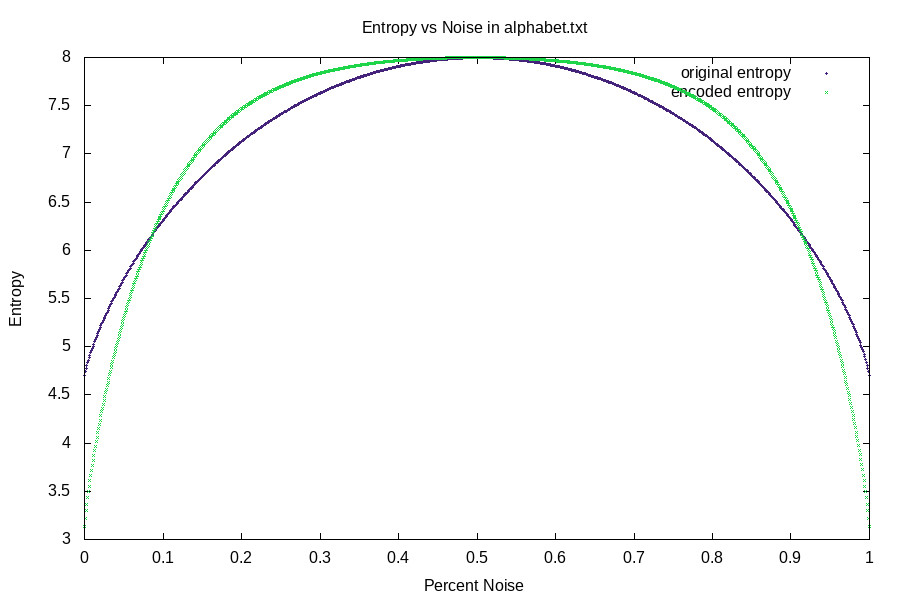
\includegraphics[width=6in]{alphabet.txt.entropy.jpg}
	\centering
\end{figure}

\begin{figure}[H]
	\caption{All As Entropy}\label{aaa_entropy}
	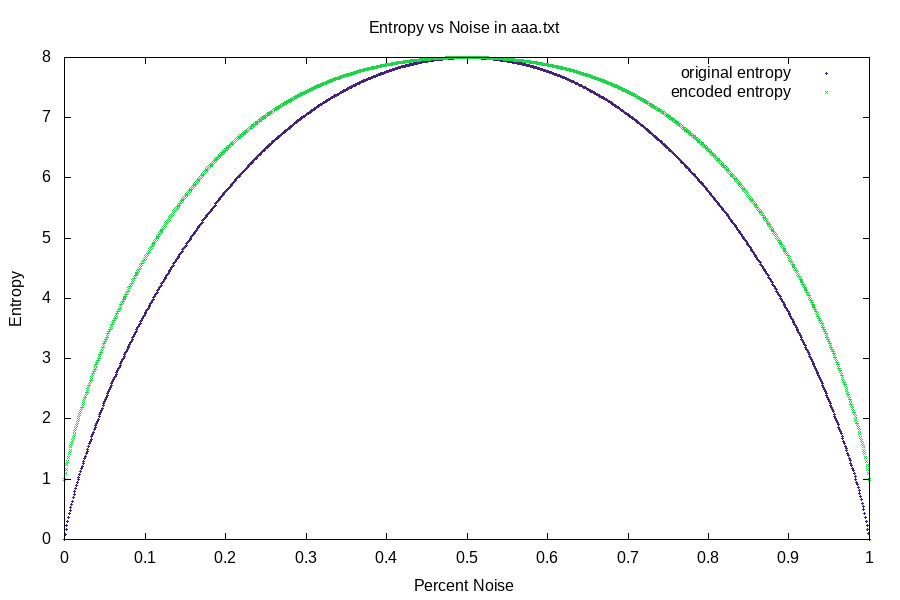
\includegraphics[width=6in]{aaa.txt.entropy.jpg}
	\centering
\end{figure}

\begin{figure}[H]
	\caption{Random Entropy}\label{random_entropy}
	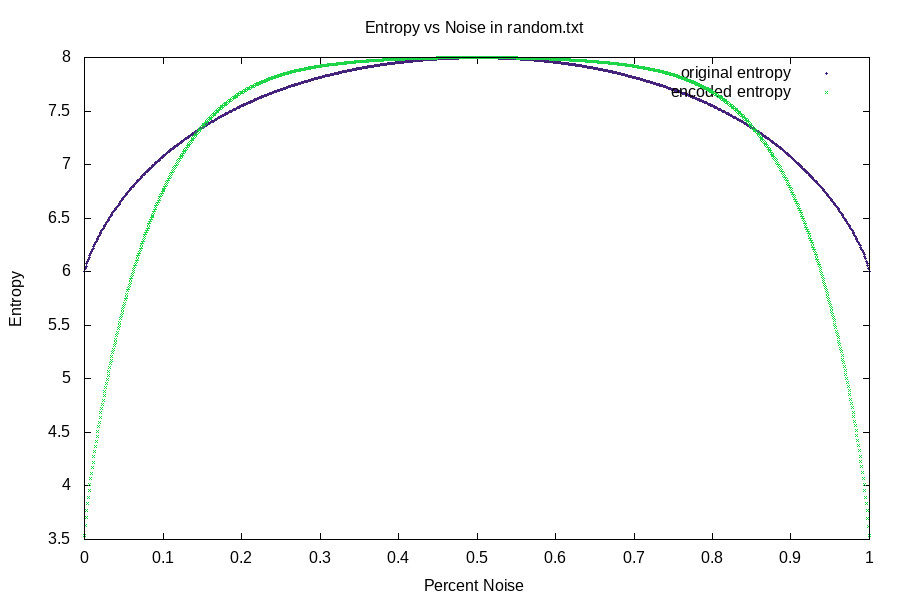
\includegraphics[width=6in]{random.txt.entropy.jpg}
	\centering
\end{figure}

\end{document}

